%%%%%%%%%%%%%%%%%%%%%%%%%%%%%%%%%%%%%%%%%%%%%%%%%
% Chapter: Events
%%%%%%%%%%%%%%%%%%%%%%%%%%%%%%%%%%%%%%%%%%%%%%%%%
\chapter{Event Notification}
\label{chap:api_event}

% RALPH
\ldots


%%%%%%%%%%%%%%%%%%%%%%%%%%%%%%%%%%%%%%%%%%%%%%
%%%%%%%%%%%%%%%%%%%%%%%%%%%%%%%%%%%%%%%%%%%%%%
\section{Logging}
\label{chap:api_event:logging}

\par
The \refapi{PMIx_Log} interface is provided to support posting information by applications and \ac{SMS} elements to persistent storage. This function is \emph{not} intended for output of computational results, streaming of raw \ac{RAS} data, or performant data operations, but rather on reporting status and saving state information (e.g., inserting computation progress reports into the application's \ac{SMS} job log). A variety of logging options are available to support use-cases such as remote monitoring of application progress (e.g., via email), output of error reports to syslog for post-mortem analysis, and caching of application completion information for use by subsequent applications in a workflow. Depending on the choice of output channel, logged information may be retrievable via the \refapi{PMIx_Query_info_nb} interface.

\par
The illustration below highlights some of the capabilities provided by the logging support. Note that the illustration is not intended to be comprehensive in its coverage as the number of possible use-cases is too large to capture in a single drawing.

\begin{figure*}[ht!]
\begin{center}
  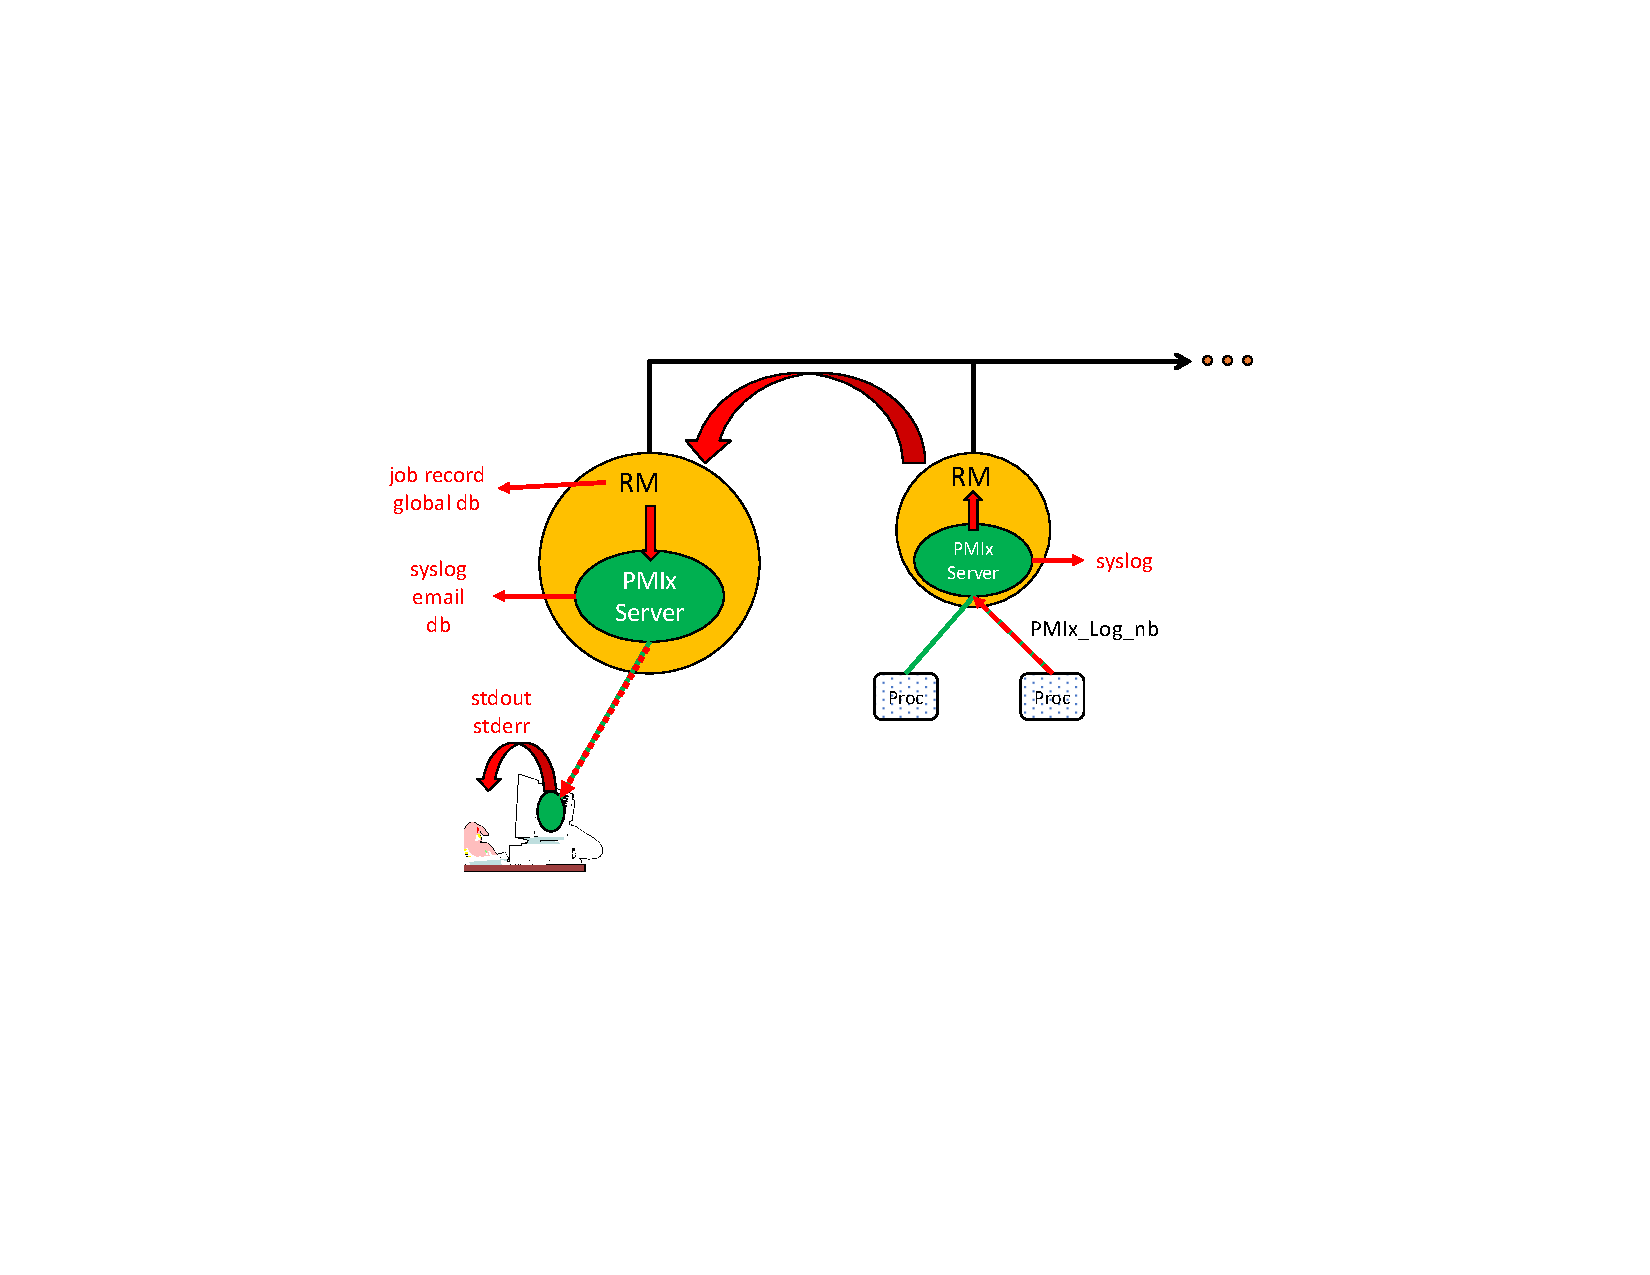
\includegraphics[clip,width=0.6\textwidth]{figs/logging.pdf}
\end{center}
  \caption{PMIx-based Logging}
  \label{fig:logging}
\end{figure*}



\par
Supported uses include:

\begin{itemize}
\item Writing of messages to syslog, both local (using the \refattr{PMIX_LOG_LOCAL_SYSLOG} attribute) or on the syslog of some central server designated for this purpose. The \ac{PMIx} client will send the logging request to its local server. If the \refattr{PMIX_LOG_LOCAL_SYSLOG} attribute is included in the request, then the \ac{PMIx} server will immediately output the message to the local syslog. If not, or if the \refattr{PMIX_LOG_GLOBAL_SYSLOG} attribute is specified, then the \ac{PMIx} server will forward the request to its host \ac{SMS} daemon. It is the responsibility of the host daemon to identify and transfer the provided data to the appropriate location --- upon arrival, the receiving daemon can use the \refapi{PMIx_Log} function to deliver the data to the local syslog on that node or can write the data to syslog itself. Attributes for setting the desired syslog priority are provided --- the default is set to to syslog priority LOG_INFO indicating reporting of an informational message

\item Sending notifications to a designated user. Application users may wish to be notified of completion of their application, receive periodic progress reports, or be notified of a problem that merits attention. \ac{PRI} includes support for some of the more popular transports --- requests for unsupported transports are referred to the host \ac{SMS} for processing, with an error returned if the requested transport is not available in the host environment

\item Outputting tagged log messages to stdout or stderr of the application, or a connected tool. Where supported, an alternative output stream (possibly directed to a dedicated log file) may be specified. Messages may be tagged (via the \refattr{PMIX_LOG_TAG_OUTPUT} attribute) as flowing via the \refattr{PMIx_Log} \ac{API} to differentiate them from the application's normal output. In addition, messages may be timestamped (\refattr{PMIX_LOG_TIMESTAMP_OUTPUT}) or output in \ac{XML} format (\refattr{PMIX_LOG_XML_OUTPUT})

\item Storing status updates in the job record using the \refattr{PMIX_LOG_JOB_RECORD} attribute. Resource managers nearly always maintain a record of the jobs they schedule and execute. This includes information on the time spent waiting for allocation, priority of the request, identity of the requestor, name/path of the executable and/or job script, etc. Historically, users have had to record status information on their application (e.g., computational progress) in files which are subsequently stored in persistent storage. \refapi{PMIx_Log} offers the option (where supported) of injecting such status reports directly into the job record, thus providing a single, time sequential record of the job's execution.

Note that system libraries can also use this feature to record job-affecting events (e.g., network failures) that might have impacted the application during its execution, perhaps linking them to more detailed information stored in a \ac{RAS} database.

\item Storing state information in a global key-value datastore. The prior use-cases all involve one-way output of data --- i.e., the caller can \emph{log} the data, but cannot later retrieve it. However, there are times when an application, tool, or \ac{SMS} element may wish to store information in a global key-value datastore that can be searched by external agents or be retrieved by the caller itself at some later time. For example, an \ac{SMS} element may wish to store state information in a persistent place for retrieval upon recovery from a failure. Use of the \refapi{PMIx_Publish} \ac{API} might, at first glance, appear to meet this need. However, \refapi{PMIx_Publish} is focused on inter/intra-application data exchange - it therefore does not guarantee persistence across (for example) an \ac{RM} failure.

Passing the \refattr{PMIX_LOG_GLOBAL_DATASTORE} attribute in a call to \refapi{PMIx_Log} indicates that the provided data is to be stored in a persistent datastore. Additional attributes can be used to provide direction on the storage strategy - e.g., hot/warm/cold or locality. Note that it is advisable to use the \emph{optional} flag for storage strategy directives as support for such behaviors is not yet commonplace.

Once logged, the data is retrievable using the \refapi{PMIx_Query_info_nb} \ac{API}. Note that the time required to retrieve the requested data will vary depending on storage location --- this is \emph{not} intended as a performant operation. Attributes to direct the behavior of the query (e.g., indicating if the caller should wait for the data to become available) are provided.
\end{itemize}

\par
Note that data can be logged without specifying the output channel. In this case, the PMIx library will default to logging a copy of the data to each available channel. The caller can optionally control the logging behavior by providing multiple channel attributes in order of desired priority, subject to the availability of the specified channel. For example, an application could ask that data be emailed to a given user, or logged to a global syslog, or logged to local syslog by specifying first the \refattr{PMIX_LOG_EMAIL} attribute, followed by the \refattr{PMIX_LOG_GLOBAL_SYSLOG} and the \refattr{PMIX_LOG_LOCAL_SYSLOG} attributes, with the \refattr{PMIX_LOG_ONCE} attribute being included to indicate that only one log channel should be used. If \refattr{PMIX_LOG_ONCE} is not indicated, then the data will be logged to all three channels. In this case, the \refattr{PMIX_ERR_PARTIAL_COMPLETION} error is returned if any channel fails to log as requested, but others succeed; \refattr{PMIX_ERR_OPERATION_FAILED} is returned if all fail; and \refattr{PMIX_SUCCESS} is returned if all succeed. This provides flexibility with minimal code complexity when operating in multiple environments that support differing output channels.

\par
Logging attributes can also utilize the ``required'' flag in the \refattr{pmix_info_t} structure to indicate that the data \emph{must} be logged via the specified channel. If given, failure to complete the operation on that channel will result in return of the \refattr{PMIX_ERR_OPERATION_FAILED} error. Otherwise, use of a given channel is considered ``optional'' and errors are reported according to the above rules.

Specifying a prioritized list of logging channels on each call to \refapi{PMIx_Log} can impact the performance of the \ac{API} itself as it requires the \ac{PMIx} library to scan available channels to create an ordered list, and this might in turn require multiple passes over the available plugins. Implementations may provide (at their discretion) environmental or other directives for reducing this overhead.

Channels that are not recognized by the \ac{PMIx} library will automatically be directed to the host \ac{SMS} daemon for processing. This allows for \ac{SMS}-proprietary channel support without committing those channel names to the \ac{PMIx} Standard.

\adviceuserstart
The available channel support on a system can be queried via the \refapi{PMIx_Query_info_nb} \ac{API} should the application developer wish to tailor their code accordingly - this will always report the channels directly supported by the \ac{PMIx} library. However, channels supported by the host \ac{SMS} will be included only if the \ac{SMS} itself supports such queries.
\adviceuserend

\adviceimplstart
A complete \ac{PMIx} implementation will respond to \refapi{PMIx_Query_info_nb} calls requesting logging channels supported by the \ac{SMS} with a comma-delimited string of channel keys - e.g., \refattr{PMIX_LOG_LOCAL_SYSLOG},\refattr{PMIX_LOG_EMAIL}.
\adviceimplend

\adviceuserstart
The \refapi{PMIx_Log} API should \emph{never} be used for streaming data as it is not a ``performant'' transport and can perturb the application since it involves the local \ac{PMIx} server and host \ac{SMS} daemon.
\adviceuserend


%%%%%%%%%%%
\subsection{\code{PMIx_Log}}
\declareapi{PMIx_Log}

%%%%
\summary

Log data to a data service.

%%%%
\format

\cspecificstart
\begin{codepar}
pmix_status_t
PMIx_Log(const pmix_info_t data[], size_t ndata,
         const pmix_info_t directives[], size_t ndirs)
\end{codepar}
\cspecificend

\begin{arglist}
\argin{data}{Array of info structures (array of handles)}
\argin{ndata}{Number of elements in the \refarg{data} array (size_t)}
\argin{directives}{Array of info structures (array of handles)}
\argin{ndirs}{Number of elements in the \refarg{directives} array (size_t)}
\end{arglist}

\begin{constantdesc}
\item \refconst{PMIX_SUCCESS} The data has been logged as requested
\item \refconst{PMIX_ERR_PARTIAL_SUCCESS} Some of the data was logged, but not all requested channels were available or supported. Note that \refconst{PMIX_SUCCESS} will be returned if no specific channels were requested and at least one channel was able to perform the specified operation.
\item \refconst{PMIX_ERR_NOT_SUPPORTED} The \ac{PMIx} implementation does not support this function, or neither the implementation nor the host {SMS} support any of the desired channels.
\end{constantdesc}

%%%%
\descr

Log data to a persistent data service/store, subject to the services offered by the host environment. The data to be logged is provided in the \refarg{data} array. The (optional) \refarg{directives} can be used to request specific storage options and direct the choice of logging channel.

\subsection{\code{PMIx_Log_nb}}
\declareapi{PMIx_Log_nb}

\cspecificstart
\begin{codepar}
pmix_status_t
PMIx_Log_nb(const pmix_info_t data[], size_t ndata,
            const pmix_info_t directives[], size_t ndirs,
            pmix_op_cbfunc_t cbfunc, void *cbdata)
\end{codepar}
\cspecificend

\begin{arglist}
\argin{data}{Array of info structures (array of handles)}
\argin{ndata}{Number of elements in the \refarg{data} array (size_t)}
\argin{directives}{Array of info structures (array of handles)}
\argin{ndirs}{Number of elements in the \refarg{directives} array (size_t)}
\argin{cbfunc}{Callback function \refapi{pmix_op_cbfunc_t} (function reference)}
\argin{cbdata}{Data to be passed to the callback function (memory reference)}
\end{arglist}

\begin{constantdesc}
\item \refconst{PMIX_SUCCESS} The logging request is valid and is being processed. The resulting status from the operation will be provided in the callback function.
\item \refconst{PMIX_ERR_BAD_PARAM} The logging request contains at least one incorrect entry that prevents it from being processed. The callback function will \emph{not} be called.
\item \refconst{PMIX_ERR_NOT_SUPPORTED} The \ac{PMIx} implementation does not support this function. The callback function will \emph{not} be called.
\end{constantdesc}

%%%%
\descr

Non-blocking version of the \refapi{PMIx_Log} routine. The callback function will be executed when the log operation has been completed. The \refarg{data} and \refarg{directives} arrays must be maintained until the callback is provided.


%%%%%%%%%%%%%%%%%%%%%%%%%%%%%%%%%%%%%%%%%%%%%%
%%%%%%%%%%%%%%%%%%%%%%%%%%%%%%%%%%%%%%%%%%%%%%
\section{Notification and Management}
\label{chap:api_event:notify}

\ldots


%%%%%%%%%%%
\subsection{\code{PMIx_Register_event_handler}}
\declareapi{PMIx_Register_event_handler}

\cspecificstart
\begin{codepar}
/* Register an event handler to report events. Three types of events
 * can be reported:
 *
 * (a) those that occur within the client library, but are not
 *     reportable via the API itself (e.g., loss of connection to
 *     the server). These events typically occur during behind-the-scenes
 *     non-blocking operations.
 *
 * (b) job-related events such as the failure of another process in
 *     the job or in any connected job, impending failure of hardware
 *     within the job's usage footprint, etc.
 *
 * (c) system notifications that are made available by the local
 *     administrators
 *
 * By default, only events that directly affect the process and/or
 * any process to which it is connected (via the PMIx_Connect call)
 * will be reported. Options to modify that behavior can be provided
 * in the info array
 *
 * Both the client application and the resource manager can register
 * err handlers for specific events. PMIx client/server calls the registered
 * err handler upon receiving event notify notification (via PMIx_Notify_event)
 * from the other end (Resource Manager/Client application).
 *
 * Multiple err handlers can be registered for different events. PMIX returns
 * an integer reference to each register handler in the callback fn. The caller
 * must retain the reference in order to deregister the evhdlr.
 * Modification of the notification behavior can be accomplished by
 * deregistering the current evhdlr, and then registering it
 * using a new set of info values.
 *
 * See pmix_common.h for a description of the notification function */
void
PMIx_Register_event_handler(pmix_status_t codes[], size_t ncodes,
                            pmix_info_t info[], size_t ninfo,
                            pmix_notification_fn_t evhdlr,
                            pmix_evhdlr_reg_cbfunc_t cbfunc,
                            void *cbdata);
\end{codepar}
\cspecificend


%%%%%%%%%%%
\subsection{\code{PMIx_Deregister_event_handler}}
\declareapi{PMIx_Deregister_event_handler}

\cspecificstart
\begin{codepar}
/* Deregister an event handler
 * evhdlr_ref is the reference returned by PMIx from the call to
 * PMIx_Register_event_handler. If non-NULL, the provided cbfunc
 * will be called to confirm removal of the designated handler */
void
PMIx_Deregister_event_handler(size_t evhdlr_ref,
                              pmix_op_cbfunc_t cbfunc,
                              void *cbdata);
\end{codepar}
\cspecificend


%%%%%%%%%%%
\subsection{\code{PMIx_Notify_event}}
\declareapi{PMIx_Notify_event}

\cspecificstart
\begin{codepar}
/* Report an event to a process for notification via any
 * registered evhdlr. The evhdlr registration can be
 * called by both the server and the client application. On the
 * server side, the evhdlr is used to report events detected
 * by PMIx to the host server for handling. On the client side,
 * the evhdlr is used to notify the process of events
 * reported by the server - e.g., the failure of another process.
 *
 * This function allows the host server to direct the server
 * convenience library to notify all registered local procs of
 * an event. The event can be local, or anywhere in the cluster.
 * The status indicates the event being reported.
 *
 * The client application can also call this function to notify the
 * resource manager of an event it encountered. It can request the host
 * server to notify the indicated processes about the event.
 *
 * The array of procs identifies the processes that will be impacted
 * by the event. This could consist of a single process, or a number
 * of processes.
 *
 * The info array contains any further info the RM can and/or chooses
 * to provide.
 *
 * The callback function will be called upon completion of the
 * notify_event function's actions. Note that any messages will
 * have been queued, but may not have been transmitted by this
 * time. Note that the caller is required to maintain the input
 * data until the callback function has been executed!
*/
pmix_status_t
PMIx_Notify_event(pmix_status_t status,
                  const pmix_proc_t *source,
                  pmix_data_range_t range,
                  pmix_info_t info[], size_t ninfo,
                  pmix_op_cbfunc_t cbfunc, void *cbdata);
\end{codepar}
\cspecificend


%%%%%%%%%%%
\subsection{Event Notification Callback Function}
\declareapi{pmix_event_notification_cbfunc_fn_t}

The \refapi{pmix_event_notification_cbfunc_fn_t} \ldots

\cspecificstart
\begin{codepar}
/* define a callback by which an event handler can notify the PMIx library
 * that it has completed its response to the notification. The handler
 * is _required_ to execute this callback so the library can determine
 * if additional handlers need to be called. The handler shall return
 * PMIX_SUCCESS if no further action is required. The return status
 * of each event handler and any returned pmix_info_t structures
 * will be added to the array of pmix_info_t passed to any subsequent
 * event handlers to help guide their operation.
 *
 * If non-NULL, the provided callback function will be called to allow
 * the event handler to release the provided info array.
 */
typedef void (*pmix_event_notification_cbfunc_fn_t)(pmix_status_t status,
                                                    pmix_info_t *results, size_t nresults,
                                                    pmix_op_cbfunc_t cbfunc, void *thiscbdata,
                                                    void *notification_cbdata);
\end{codepar}
\cspecificend

%%%%
\descr

\ldots


%%%%%%%%%%%
\subsection{Notification Callback Function}
\declareapi{pmix_notification_fn_t}

The \refapi{pmix_notification_fn_t} \ldots

\cspecificstart
\begin{codepar}
/* define a callback function for the event handler. Upon receipt of an
 * event notification, PMIx will execute the specified notification
 * callback function, providing:
 *
 * evhdlr_registration_id - the returned registration number of
 *                          the event handler being called
 * status - the event that occurred
 * source - the nspace and rank of the process that generated
 *          the event. If the source is the resource manager,
 *          then the nspace will be empty and the rank will
 *          be PMIX_RANK_UNDEF
 * info - any additional info provided regarding the event.
 * ninfo - the number of info objects in the info array
 * results - any provided results from event handlers called
 *           prior to this one.
 * nresults - number of info objects in the results array
 * cbfunc - the function to be called upon completion of the handler
 * cbdata - pointer to be returned in the completion cbfunc
 *
 * Note that different resource managers may provide differing levels
 * of support for event notification to application processes. Thus, the
 * info array may be NULL or may contain detailed information of the event.
 * It is the responsibility of the application to parse any provided info array
 * for defined key-values if it so desires.
 *
 * Possible uses of the pmix_info_t object include:
 *
 * - for the RM to alert the process as to planned actions, such as
 *   to abort the session, in response to the reported event
 *
 * - provide a timeout for alternative action to occur, such as for
 *   the application to request an alternate response to the event
 *
 * For example, the RM might alert the application to the failure of
 * a node that resulted in termination of several processes, and indicate
 * that the overall session will be aborted unless the application
 * requests an alternative behavior in the next 5 seconds. The application
 * then has time to respond with a checkpoint request, or a request to
 * recover from the failure by obtaining replacement nodes and restarting
 * from some earlier checkpoint.
 *
 * Support for these options is left to the discretion of the host RM. Info
 * keys are included in the common definions above, but also may be augmented
 * on a per-RM basis.
 *
 * On the server side, the notification function is used to inform the host
 * server of a detected event in the PMIx subsystem and/or client
 */
typedef void (*pmix_notification_fn_t)(size_t evhdlr_registration_id,
                                       pmix_status_t status,
                                       const pmix_proc_t *source,
                                       pmix_info_t info[], size_t ninfo,
                                       pmix_info_t *results, size_t nresults,
                                       pmix_event_notification_cbfunc_fn_t cbfunc,
                                       void *cbdata);
\end{codepar}
\cspecificend

%%%%
\descr

\ldots



%%%%%%%%%%%
\subsection{Event Handler Registration Function}
\declareapi{pmix_evhdlr_reg_cbfunc_t}

The \refapi{pmix_evhdlr_reg_cbfunc_t} \ldots

\cspecificstart
\begin{codepar}
/* define a callback function for calls to PMIx_Register_evhdlr. The
 * status indicates if the request was successful or not, evhdlr_ref is
 * an integer reference assigned to the event handler by PMIx, this reference
 * must be used to deregister the err handler. A ptr to the original
 * cbdata is returned. */
typedef void (*pmix_evhdlr_reg_cbfunc_t)(pmix_status_t status,
                                         size_t evhdlr_ref,
                                         void *cbdata)
\end{codepar}
\cspecificend

%%%%
\descr

\ldots


%%%%%%%%%%%%%%%%%%%%%%%%%%%%%%%%%%%%%%%%%%%%%%%%%
